\documentclass[twoside,10pt]{article}
\usepackage{amsmath,amsfonts,amsthm,fullpage}
\usepackage{algorithm}
\usepackage{algorithmic}
\usepackage{graphicx}


\begin{document}

\title{ISYE 6740 Spring 2022\\ Homework 1 (100 points + 5 bonus points)}
%\author{Yao Xie}
\date{}

\maketitle

\vspace{-.5in}

%In this homework, the superscript of a symbol $\text x^i$ denotes the index of samples (not raising to $i$th power); this is a convention in this class. 

\section{Concept questions [30 points]}

Please provide a brief answer to each question.

\begin{enumerate}

\item (5 points) What's the main difference between supervised and unsupervised learning?

\item (5 points) Will different initializations for k-means lead to different results?

\item (5 points) Give a short proof (can be in words but using correct logic) why k-means algorithm will converge in finite number of iterations.

\item (5 points) What is the main difference between k-means and generalized k-means algorithm? Explain how the choice of the similarity/dissimilarity/distance will impact the result. 



\item (10 points) Consider the following simple graph
\begin{center}
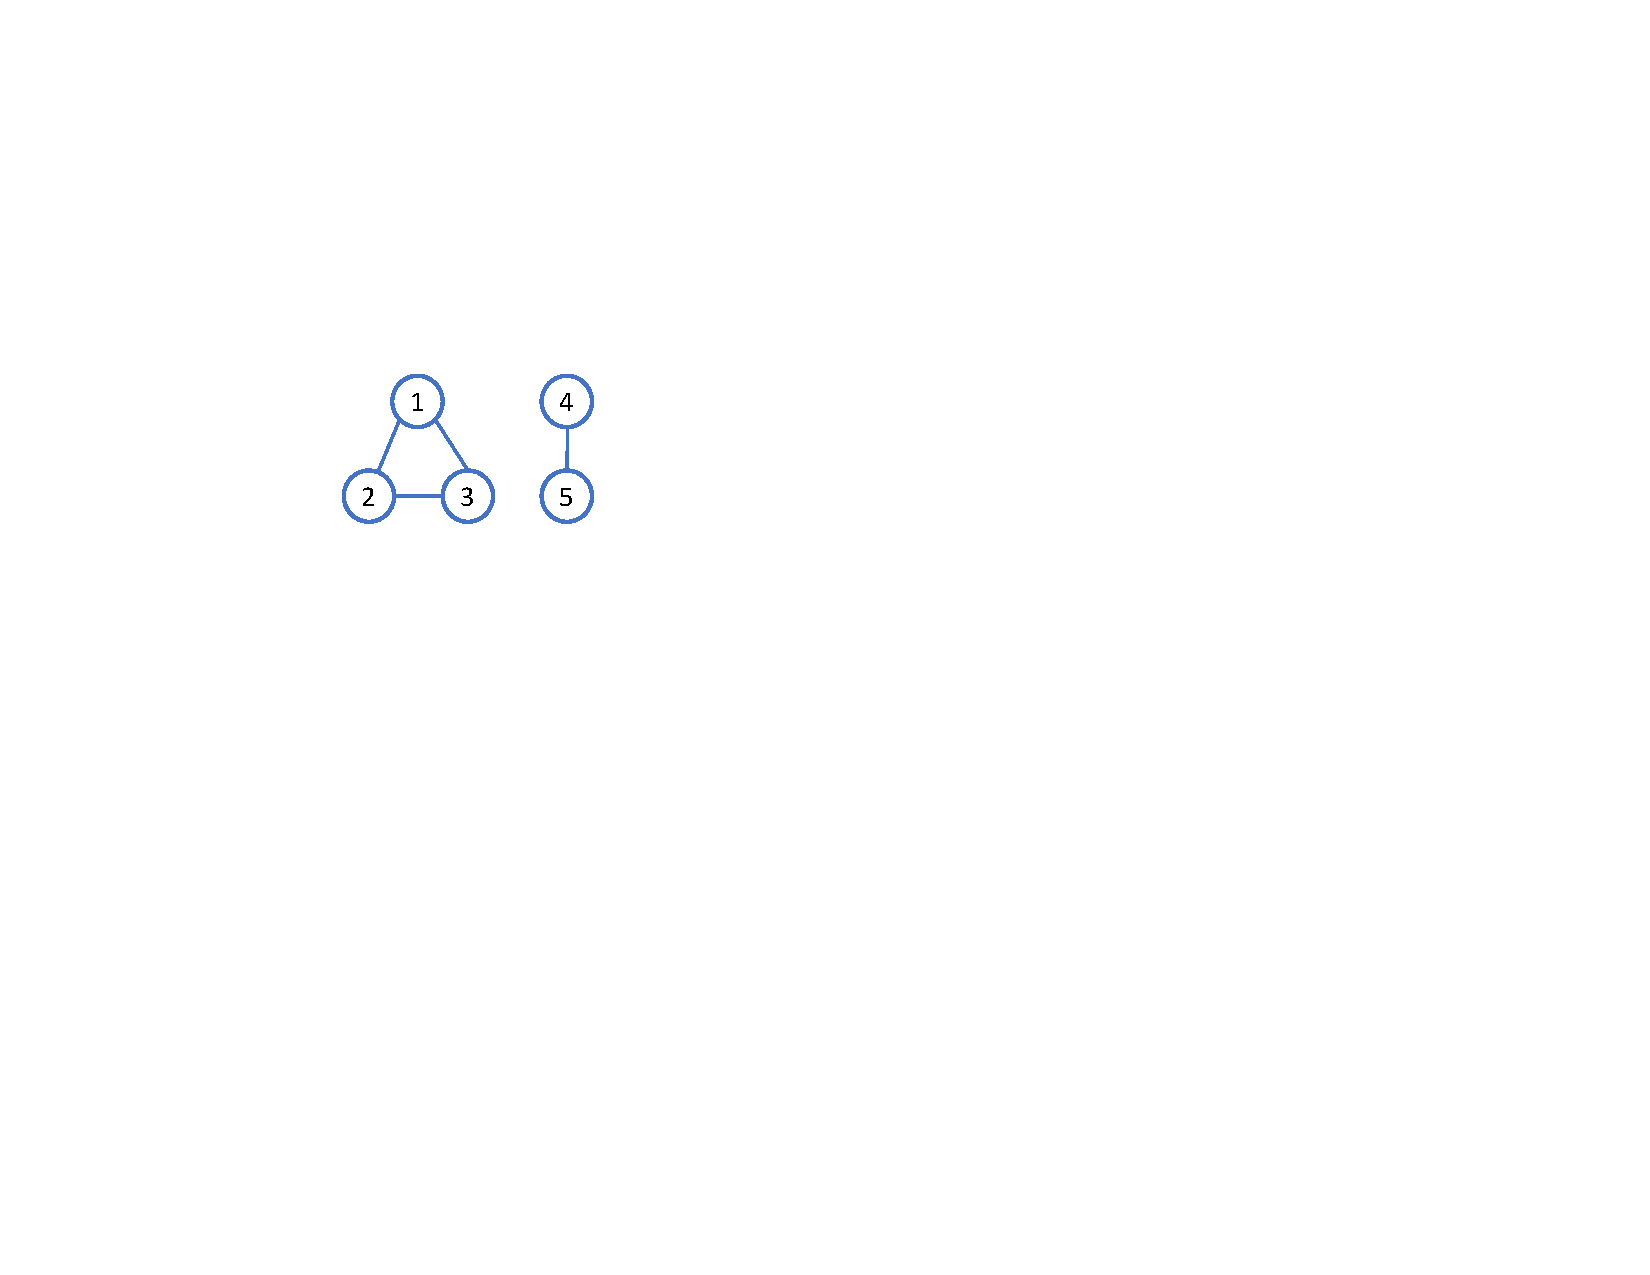
\includegraphics[width = 0.2\textwidth]{plot}
\end{center}

Write down the graph Laplacian matrix and find the eigenvectors associated with the zero eigenvalue. Explain how do you find out the number of disconnected clusters in graph and identify these disconnected clusters using these eigenvectors.

\end{enumerate}


\section{Image compression using clustering [40 points]}

In this programming assignment, you are going to apply clustering algorithms for image compression. Your task is to implement \emph{$K$-means} for this purpose.  {\bf It is required you implement the algorithms yourself rather than calling k-means from a package. However, it is ok to use standard packages for supplementary tasks, e.g. file i/o, linear algebra, and visualization.} 


\subsubsection*{Formatting instruction}

As a starting point, we suggest the following input/output signature for your k-means algorithm.\\

\textbf{Input}
\begin{itemize}
  \item \texttt{pixels}: the input image representation. Each row contains one data point (pixel). For image dataset, it contains 3 columns, each column corresponding to Red, Green, and Blue component. Each component has an integer value between 0 and 255.
  \item \texttt{k}: the number of desired clusters.
\end{itemize}

\textbf{Output}
\begin{itemize}
  \item \texttt{class}: cluster assignment of each data point in pixels. The assignment should be 1, 2, 3, etc. For $k = 5$, for example, each cell of class should be either 1, 2, 3, 4, or 5. The output should be a column vector with \texttt{size(pixels, 1)} elements.
  \item \texttt{centroid}: location of $k$ centroids (or representatives) in your result. With images, each centroid corresponds to the representative color of each cluster. The output should be a matrix with $K$ rows and 3 columns. The range of values should be [0, 255], possibly floating point numbers.
\end{itemize}

\subsubsection*{Hand-in}
Both of your code and report will be evaluated. Upload the code as a zip file, and the report as a pdf, separately from the zip file. In your report, answer to the following questions:
\begin{enumerate}
  \item (20 points) Use $k$-means with squared-$\ell_2$ norm as a metric, for \texttt{GeorgiaTech.bmp} and \texttt{football.bmp} and also choose a third picture of your own to work on. We recommend size of $320 \times 240$ or smaller. Run your $k$-means implementation with these pictures, with several different $k = 2, 4, 8, 16$. 
  
  
Run your $k$-means implementation (with squared-$\ell_2$ norm) with random initialization centroids. Please try multiple time and report the best one (in terms of the image quality).
  
Please write in your report, how long does it take to converge for each $k$ (report the number of iterations, and elapsed time in seconds) and also include the resulted compressed pictures for each $k$ \textbf{in the report}.
  
\item (20 points) Now try your $k$-means with the Manhattan distance (or $\ell_1$ distance) and repeat the same steps in Part (1). Please note that the assignment of data point should be based on the Manhattan distance, and the cluster centroid (by minimizing the sum of deviance -- as a result of using the Manhattan distance) will be taken as the ``median'' of each cluster. Comment on the difference of image compression results using the two methods.
   
\end{enumerate}


\subsubsection*{Note}
\begin{itemize}
  \item You may see errors caused by empty clusters when you use too large $k$. Your implementation should treat this exception as well. That is, do not terminate even if you have an empty cluster, but automatically decrement to a smaller number of clusters.

  \item We recommend you to test your code with several different pictures so that you can detect some problems that might happen occasionally. 

  \item If we detect plagarism from any other student's code or from the web, you will not be eligible for any credit for the entire homework, not just for this problem.
\end{itemize}



\section{Political blogs dataset [30 points]}

We will study a political blogs dataset first compiled for the paper Lada A. Adamic and Natalie Glance, ``The political blogosphere and the 2004 US Election'', in Proceedings of the WWW-2005 Workshop on the Weblogging Ecosystem (2005). It is assumed that blog-site with the same political orientation are more likely to link to each other, thus, forming a ``community'' or ``cluster'' in a graph. In this question, we will see whether or not this hypothesis is likely to be true based on data.
\begin{itemize}

\item The dataset \textsf{nodes.txt} contains a graph with $n = 1490$ vertices (``nodes'') corresponding to political blogs. 

\item The dataset \textsf{edges.txt} contains edges between the vertices. You may remove isolated nodes (nodes that are not connected any other nodes) in the pre-processing. 

\end{itemize}

We will treat the network as an undirected graph; thus, when constructing the adjacency matrix, make it symmetrical by, e.g., set the entry in the adjacency matrix to be one whether there is an edge between the two nodes (in either direction). 

In addition, each vertex has a 0-1 label (in the 3rd column of the data file) corresponding to the true political orientation of that blog. We will consider this as the true label and check whether spectral clustering will cluster nodes with the same political orientation as possible. 

\begin{enumerate}

\item (15 points) Use spectral clustering to find the $k = 2, 5, 10, 20$ clusters in the network of political blogs (each node is a blog, and their edges are defined in the file \textsf{edges.txt}). Find majority labels in each cluster, for different $k$ values, respectively. For example, if there are $k = 2$ clusters, and their labels are $\{0, 1, 1, 1\}$ and $\{0, 0, 1\}$ then the majority label for the first cluster is 1 and for the second cluster is 0. {\bf It is required you implement the algorithms yourself rather than calling from a package.} 

Now compare the majority label with the individual labels in each cluster, and report the {\it mismatch rate} for each cluster, when $k = 2, 5, 10, 20$. For instance, in the example above, the mismatch rate for the first cluster is 1/4 (only the first node differs from the majority) and the the second cluster is 1/3. 

\item (15  points) Tune your $k$ and find the number of clusters to achieve a reasonably small {\it mismatch rate}. Please explain how you tune $k$ and what is the achieved mismatch rate. Please explain intuitively what this results tells about the network community structure.

\end{enumerate}

\section{(Bonus Question) Math of k-means clustering [5 points]}

Given $m$ data points $\text x^i$, $i=1,\dots, m$, $K$-means clustering algorithm groups them into $k$ clusters by minimizing the distortion function over $\{ r^{ij}, \mu^j \}$
\begin{equation}
J =\sum_{i=1}^m\sum_{j=1}^k r^{ij} \|\text x^i-\mu^j\|^2,
\label{J_def}
\end{equation}
where $r^{ij}=1$ if $\text x^i$ belongs to the $j$-th cluster and $r^{ij}=0$ otherwise.

\begin{enumerate}

\item (3 points) Derive mathematically that using the squared Euclidean distance $\|\text x^i-\mu^j\|^2$ as the dissimilarity function, the centroid that minimizes the distortion function $J$  for given assignments $r^{ij}$ are given by
   $$\mu^j=\frac{\sum_i r^{ij} \text x^i}{\sum_i r^{ij}}.$$
   That is, $\mu^j$ is the center of $j$-th cluster.  \\
   Hint: You may start by taking the partial derivative of $J$ with respect to $\mu^j$, with $r^{ij}$ fixed.
   
   
\item (2 points) Derive mathematically what should be the assignment variables $r^{ij}$ be to minimize the distortion function $J$, when the centroids $\mu^j$ are fixed.

\end{enumerate}


\end{document}
